\documentclass{jlreq}

\usepackage{titlesec}
\usepackage{listings}
\usepackage{fancyhdr}

% url
\usepackage{url}

% \adjustbox
\usepackage{adjustbox}

% tcolorboxの設定
\usepackage[most]{tcolorbox} 
\tcbuselibrary{breakable}
\tcbuselibrary{skins}
\tcbuselibrary{listingsutf8}
% タイトルのフォーマットを変更
\titleformat{\title}
  {\centering\Huge\bfseries}
  {}
  {0em} 
  {}

\titleformat{\subtitle}
  {\centering\Large\itshape}
  {}
  {0em}
  {}

\titleformat{\subsubsection}[block]
  {\normalfont\normalsize\bfseries}
  {\arabic{subsubsection}.}
  {1em}
  {}

\titleformat{\section}[block]
  {\normalfont\large\bfseries}
  {\Roman{section}.}
  {1em} 
  {}
  [\titleline{\titlerule[1pt]}]

\titleformat{\subsection}[block]
  {\normalfont\normalsize\bfseries}
  {\roman{subsection}.}
  {1em}
  {}

% listingsの設定

\renewcommand{\lstlistingname}{コード}

\lstset{
	breaklines = true,
	language = Python,
	keywordstyle = {\bfseries \color[cmyk]{0,1,0,0}},
	commentstyle = {\itshape \color[cmyk]{1,0.4,1,0}},
	numbers = left,
	numberstyle = \tiny,
	stepnumber = 1,
	% frameとnumberの間の距離
	numbersep = 10pt,
	frame = single,
	basicstyle = \ttfamily,
	tabsize = 2,
	captionpos = t,
	backgroundcolor={\color[gray]{.90}},
	showstringspaces = false,
}

% headerの設定
\pagestyle{fancy}
\fancyhf{}

\fancyhead[RO,RE]{\rightmark}
\fancyhead[LO,LE]{\leftmark} 
\fancyfoot[C]{\thepage}

% tikzの設定
\usepackage{tikz}

\begin{document}
探索の章で扱うアルゴリズムは以下と通りです。

\begin{itemize}
  \item 線形探索
  \item 二分探索
  \item 二分探索木
  \item Treeq
  \item 平衡木(AVL木、B木、赤黒木)
  \item ハッシュ法
\end{itemize}

検索(サーチ)とは、データ集合(配列など)から、目的とする値を持った要素を探し出すことを意味する。

\section{線形探索}

\textbf{線形探索}は、目的とする要素が見つかるまで先頭から順に要素を見ていく探索方法です。例えば、以下の配列で0を探すなら前から順番に、
8, 4, 5, 0, 2の順に要素を見ていきます。

\vspace{0.5cm}

\begin{center}
  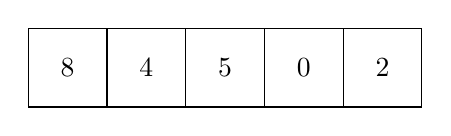
\begin{tikzpicture}
      \draw (0, 0) rectangle (1, 1);
      \node at (0.5, 0.5) {8};
      
      \draw (1, 0) rectangle (2, 1);
      \node at (1.5, 0.5) {4};
      
      \draw (2, 0) rectangle (3, 1);
      \node at (2.5, 0.5) {5};
      
      \draw (3, 0) rectangle (4, 1);
      \node at (3.5, 0.5) {0};
      
      \draw (4, 0) rectangle (5, 1);
      \node at (4.5, 0.5) {2};
  \end{tikzpicture}
\end{center}

\subsection{線形探索の実装}
\begin{lstlisting}[caption=線形探索の実装, frame=TRBL, label={linear}]
def linear_search(array: list[int], value: int) -> int:
    """
    線形探索をして一致するならそのindexを返す. 一致しないときは-1を返す
    """
    for i in range(len(array)):
        if array[i] == value:
            return i
    
    return -1


\end{lstlisting}

\subsection{番兵}

番兵法では探索するデータ集合の最後に目的とする数を追加します。最後に番兵を追加することで、より効率的に探索を行うことができます。
実際には番兵を追加してもそこまで効率が良くなるわけではないですが、番兵を追加することで、ループの条件判定を省略することができます。

\vspace{0.5cm}

\begin{center}
  \begin{tikzpicture}
      \draw (0, 0) rectangle (1, 1);
      \node at (0.5, 0.5) {8};
      
      \draw (1, 0) rectangle (2, 1);
      \node at (1.5, 0.5) {4};
      
      \draw (2, 0) rectangle (3, 1);
      \node at (2.5, 0.5) {5};
      
      \draw (3, 0) rectangle (4, 1);
      \node at (3.5, 0.5) {3};
      
      \draw (4, 0) rectangle (5, 1);
      \node at (4.5, 0.5) {2};
      
      \draw (5, 0) rectangle (6, 1);
      \fill[red, overlay] (5, 0) rectangle (6, 1);
      \node[white] at (5.5, 0.5) {0};
      \node[] at (5.5, -0.5) {番兵};
  \end{tikzpicture}
\end{center}

\begin{lstlisting}[caption=番兵の実装, frame=TRBL, label={sentinel}]
def linear_search(array: list[int], value: int) -> int:
    """
    線形探索をして一致するならそのindexを返す. 一致しないときは-1を返す
    """
    i = 0
    copied_array = array.copy()
    copied_array.append(value)
    while copied_array[i] != value: i += 1
    
    return i if i < len(array) else -1
  \end{lstlisting}

\section{二分探索}
\begin{center}
  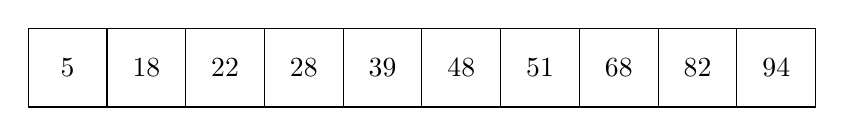
\begin{tikzpicture}
      \draw (0, 0) rectangle (1, 1);
      \node at (0.5, 0.5) {5};
      
      \draw (1, 0) rectangle (2, 1);
      \node at (1.5, 0.5) {18};
      
      \draw (2, 0) rectangle (3, 1);
      \node at (2.5, 0.5) {22};
      
      \draw (3, 0) rectangle (4, 1);
      \node at (3.5, 0.5) {28};
      
      \draw (4, 0) rectangle (5, 1);
      \node at (4.5, 0.5) {39};
      
      \draw (5, 0) rectangle (6, 1);
      \node at (5.5, 0.5) {48};
      
      \draw (6, 0) rectangle (7, 1);
      \node at (6.5, 0.5) {51};
      
      \draw (7, 0) rectangle (8, 1);
      \node at (7.5, 0.5) {68};
      
      \draw (8, 0) rectangle (9, 1);
      \node at (8.5, 0.5) {82};
      
      \draw (9, 0) rectangle (10, 1);
      \node at (9.5, 0.5) {94};
  \end{tikzpicture}
\end{center}

\newpage

\section{参考}
\textbf{二分探索}

\begin{itemize}
  \item \url{https://qiita.com/drken/items/97e37dd6143e33a64c8c}
\end{itemize}


\end{document}